\documentclass{article}
\usepackage{graphicx}
\title{Assignment 0}
\author{Tore Kjelds (tokj@itu.dk)}
\date{\today}

\begin{document}
\maketitle
\section*{Leap Year Documentation}
\begin{figure}[!htb]
    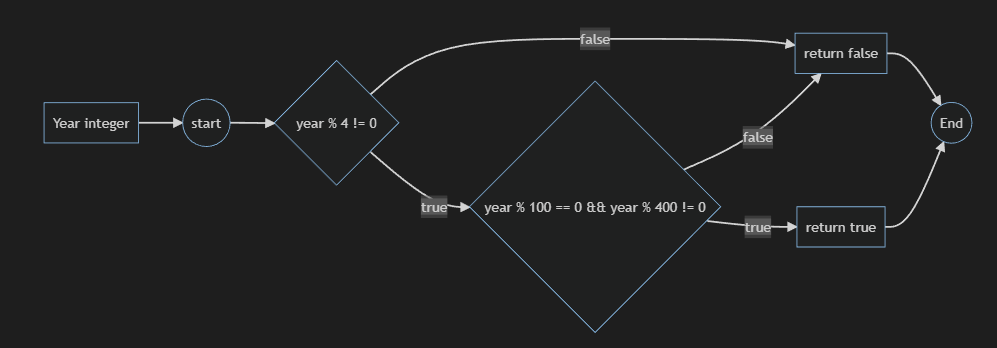
\includegraphics[scale = 0.5]{img/Flowchart_Leap_Year.png}
\end{figure}

\begin{itemize}
    \item The algorithm starts when it is given an integer as input.
    \item Therafter it checks whether or not the input is wholely divisible by 4. 
    \begin{itemize}
        \item if it is not, the algorithm ends and returns false.
        \item if it is, the algorithm continues on to the next step
    \end{itemize}
    \item The algorithm then checks if the input is wholely divisible with 100 and if the input is not wholely divisible with 400.
    \begin{itemize}
        \item If it does not fulfill the checks, the algorithm ends and returns false
        \item If it fulfills the checks the algorithm ends and returns true
    \end{itemize}
\end{itemize}
\end{document}
